\documentclass[a4paper, 10pt]{article}
\usepackage[spanish] {babel}
\title{Trabajo Practico 1}
\usepackage{floatflt}
\usepackage{tporga2}
\usepackage{caratula}
\usepackage[pdftex]{graphicx}
\usepackage{color}

\setlength{\leftmargin}{2cm}
\setlength{\rightmargin}{2cm}
\setlength{\oddsidemargin}{-1cm}
\setlength{\evensidemargin}{-1cm}
\setlength{\topmargin}{-1cm}
\setlength{\textwidth}{18cm}
\setlength{\textheight}{25cm}

\usepackage{fancyhdr}
\pagestyle{fancy}
\fancyhf{}
\fancyhead [LO,LE]{\scriptsize Trabajo Pr\'actico N$^{\circ}$1}
\fancyhead [RO,RE]{\scriptsize Mancuso, Mataloni, Villaverde}
\fancyfoot[CE,CO]{\thepage}
\renewcommand{\footrulewidth}{0.4pt}

\usepackage[pdftex, bookmarks=true, colorlinks, citecolor=black, linkcolor=black]{hyperref}
\usepackage{multirow}
\usepackage{listings}

\begin{document}


\materia{Organizaci\'on del Computador II}
\submateria{Segundo Cuatrimestre de 2009}
\titulo{Trabajo Practico N$^{\circ}$1}
\grupo{Grupo RET}
\integrante{Mancuso Emiliano}{597/07}{emiliano.mancuso@gmail.com}
\integrante{Villaverde Bacskay Romina}{740/07}{romina.villaverde@gmail.com}
\integrante{Mataloni Alejandro}{706/07}{amataloni@gmail.com}
\maketitle
\newpage

\addcontentsline{toc}{section}{\'Indice}
\tableofcontents

\newpage

\section{Enunciado}

Hacer un programa para el procesamiento simple de im\'agenes. El programa debe permitir cargar una imagen directamente en escala de grises, aplicar los operadores de derivaci\'on de Roberts, Prewitt y de Sobel para realzar los bordes y guardar la imagen en alg\'un formato que prefieran. Debe estar programado de manera modular, para que sea f\'acil agregar otros tipos de procesamiento en el futuro. 

Se debe escribir la parte de interacci\'on con el usuario y manejo de archivos en lenguaje C, utilizando la librer\'ia OpenCV. Las funciones de procesamiento de im\'agenes deben estar escritas en lenguaje ensamblador. El programa debe recibir en la l\'inea de comandos el nombre del archivo de entrada y la operaci\'on:

\begin{itemize}
\item r1 = realzar los bordes con el operador de Roberts.
\item r2 = realzar los bordes con el operador de Prewitt. 
\item r3 = realzar los bordes con el operador de Sobel, derivaci\'on s\'olo en x.
\item r4 = realzar los bordes con el operador de Sobel, derivaci\'on s\'olo en y.
\item r5 = realzar los bordes con el operador de Sobel, derivaci\'on en x y en y.
\end{itemize}

El prototipo de la funci\'on de realzar bordes escrita en lenguaje ensamblador debe ser: \\

\texttt{void asmSobel(const char* src, char* dst, int ancho, int alto, int xorder, int yorder);} \\

Tambi\'en se debe comparar los tiempos de ejecuci\'on entre el operador de Sobel implementado por el grupo y el operador de Sobel implementado en la librer\'ia.

\section{Implementaci\'on de los algoritmos}

Para resolver el problema de la detecci\'on de bordes lo que hicimos en un primer momento fue plantear un algoritmo que recorr\'ia la imagen a la que le quer\'iamos detectar los bordes y para cada pixel realizabamos un ciclo en el cual multiplic\'abamos la matriz de derivaci\'on por los puntos de la imagen y luego de saturar el resultado lo guard\'abamos en el lugar correspondiente de la matriz de destino. Para esto ten\'iamos definidas en C las matrices correspondientes para cada operador, las cuales eran globales por lo que las acced\'iamos desde el c\'odigo de assembler. \\ 

En las primeras versiones recorr\'iamos en un ciclo todos los valores de la matriz de convoluci\'on, y realiz\'abamos las operaciones de manera ``convencional", multiplicando los valores correspondientes de cada matriz (la de la imagen y la de los convoluci\'on) y sum\'ando el resultado a un acumulador. 

Pero luego de hacer varias consultas nos dimos cuenta que estabamos realizando operaciones de m\'as y desaprovechando espacio. Por un lado, si ya sabemos de antemano el tama\~{n}o de la matriz, no nos conven\'ia hacer un ciclo para recorrerla y realizar los c\'alculos (gastando registros y haciendo comparaciones para ver si hab\'iamos recorrido todos los valores), sino que acced\'iamos directamente a cada una de las posiciones de la matriz, hasta calcular todos los valores necesarios.

Otra mejora que hicimos fue que, aprovech\'andonos tambi\'en que conoc\'iamos los valores que ten\'ian las matrices de convoluci\'on, dejamos de multiplicar los valores de la imagen con aquellas posiciones de la matriz de convoluci\'on en las que hab\'ian 0s y 1s; con este cambio, y dependiendo del operador, nos ahorramos entre un 50 y un 66\% de los c\'alculos.

Sin embargo, con las modificaciones mencionadas anteriormente segu\'iamos desperdiciando espacio, ya que al conocer los valores que tiene cada matriz, y al no tener un ciclo que la recorra, pod\'iamos simplemente realizar las operaciones con los valores (que ya conoc\'iamos) en lugar de guardar la matriz en memoria. \'Esto tambi\'en nos ahorraba accesos a memoria, ya que con esta nueva implementaci\'on, usamos par\'ametros inmediatos en las instrucciones. \\

\newpage

\textquestiondown C\'omo realizamos las operaciones para entre los valores de cada matriz?:
\begin{itemize}
\item Como dijimos anteriormente, obviamos todos aqu\'ellas posiciones de la matriz de convoluci\'on en las que haya un 0. Es decir, en base a las modificaciones que realizamos, no tenemos en cuenta los valores nulos de la matriz, ya que tampoco incrementan el acumulador.
\item Para multiplicar por 1, simplemente sumamos al acumulador el valor correspondiente de la matriz de la imagen.
\item Para multiplicar por -1, simplemente restamos al acumulador el valor correspondiente de la matriz de la imagen.
\item Para multiplicar por 2, utilizamos la instrucci\'on SAL y sumamos el resultado al acumulador.
\item Para multiplicar por -2, utilizamos nuevamente la instrucci\'on SAL y restamos el resultado al acumulador. Podemos garantizar que esto funciona correctamente, ya que los valores de la matriz de la imagen son n\'umeros positivos. \\
\end{itemize}

Como trabajamos con una matriz con n\'umeros de ocho bits sin signo, luego de calcular el resultado por medio de la matriz de convoluci\'on, deb\'iamos saturarlo. Esto significa que si el resultado que obtuvimos fue mayor que 255, entonces deb\'iamos poner 255 en la matriz resultado (11111111 en binario). Por el contrario el resultado podia ser negativo, por lo que deb\'iamos saturar a 0 si esto suced\'ia. Para esto usamos un macro al cual le pasabamos un registro (el n\'umero al que le quer\'iamos aplicar la saturaci\'on) y nos devolv\'ia el resultado en eax (en realidad en al que es lo que nesecitabamos). \\ 

\begin{tabular}{p{6cm}l}
\texttt{\% macro saturar 1} & ;escribe en EAX el resultado de la saturacion \\
& \\

\hspace*{8mm}\texttt{cmp \%1, 255} & ;comparamos con 255 \\
\hspace*{8mm}\texttt{jnl \% \%poner255} & ;si es mayor que 255 saturo con 255 \\
& \\

\hspace*{8mm}\texttt{cmp \%1, 0} & ;comparamos con 0 \\
\hspace*{8mm}\texttt{jl \% \%ponerCero} & ; si es menor a 0 saturo con 0 \\
& \\
	
\hspace*{8mm}\texttt{mov eax, \%1} & ;si esta entre 0 y 255 pongo el mismo registro \\
\hspace*{8mm}\texttt{jmp \% \%fin}  &  \\
& \\
	
\texttt{\% \%ponerCero:} & \\
\hspace*{8mm}\texttt{mov eax, 0} &  \\
\hspace*{8mm}\texttt{jmp \% \%fin} &  \\
& \\

\texttt{\% \%poner255:} &  \\
\hspace*{8mm}\texttt{mov eax, 255} &  \\
& \\

\texttt{\% \%fin:} &  \\
& \\

\texttt{\%endmacro} &  \\	
\end{tabular}

\newpage

\section{Comparaci\'on de nuestros algoritmos}
Despues de aplicar las optimizaciones, obviamente quisimos comprobar que realmente lo eran.
Entonces utilizamos nuestro viejo algoritmo, que accedia a memoria, contra nuestro nuevo algoritmo que tiene las instrucciones inmediatas, y obtuvimos los siguientes resultados.

\begin{center}
	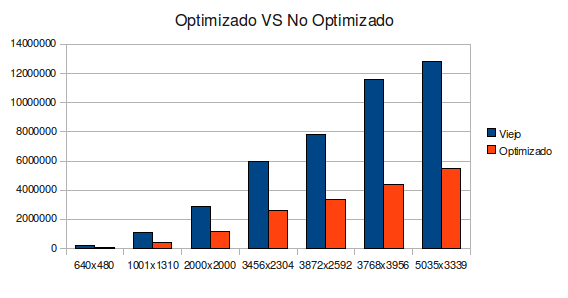
\includegraphics[scale=0.60]{Graficos/ViejoVSOptimizado.png}
\end{center}

Es notable la diferencia entre las dos implementaciones, las optimizaciones que ralizamos fueron acertadas.


\section{OpenCV vs. RET}

La librer\'ia OpenCV implementa su propio algoritmo para el operador de Sobel.
Como nosotros tambi\'en implementamos uno utilizamos im\'agenes de distintos tama\~nos, y medimos los ciclos del CPU para comparar la eficiencia de las distintas implementaciones.
Para esta comparaci\'on utilizamos nuestro algoritmo optimizado.

\begin{center}
	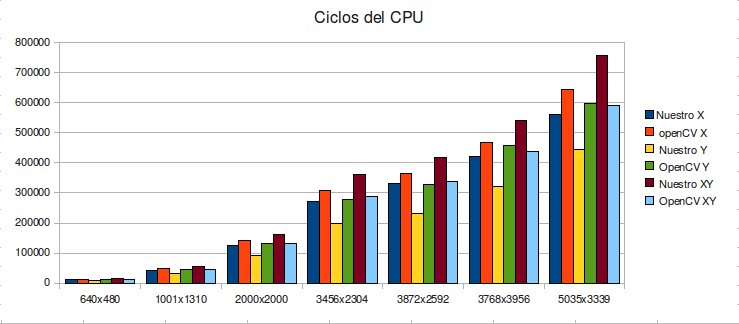
\includegraphics[scale=0.60]{Graficos/ciclosCPU.png}
\end{center}

Para realizar este gr\'afico, seleccionamos distintas im\'agenes con distinta resoluci\'on, y corrimos cada algoritmo un total de 30 veces para luego calcular un promedio.
Para ajustar la escala del gr\'afico, la cantidad de ciclos esta representada en miles, pues sino se hac\'ia despreciable respecto a las im\'agenes m\'as peque\~nas. \\ 

Con est\'e gr\'afico observamos que en im\'agenes peque\~nas las dos implementaciones eran similares, pero a medida que el tama\~no de las im\'agenes aumenta, la diferencia entre las dos se hace m\'as grande.
Si bien nuestra implementaci\'on para la derivaci\'on en X y en Y por separado consume muchos menos ciclos de CPU que la implementaci\'on de OpenCV, la librer\'ia desarrollo un algoritmo mucho m\'as eficiente para la detecci\'on de los bordes en XY.

\newpage

\section{Imagenes procesadas}

Para probar los algoritmos, y los distintos operadores, tomamos la siguiente fotograf\'ia.

\begin{center}
	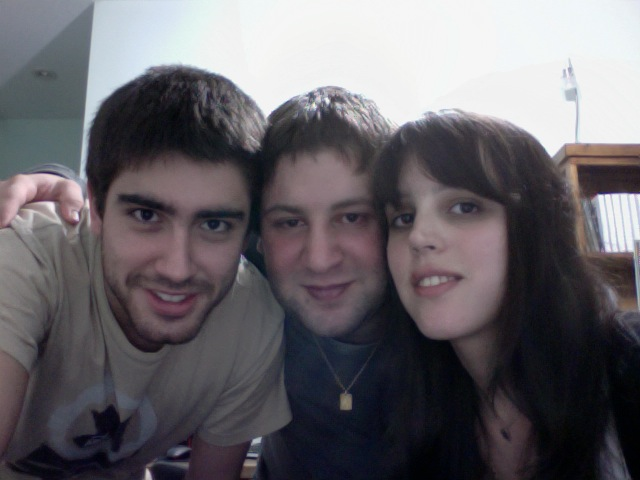
\includegraphics[scale=0.30]{Graficos/out/foto3.jpg}
\end{center}

Conforme a los operadores especificados, obtuvimos los siguientes resultados.

\subsection{Operador de Roberts}

\begin{center}
	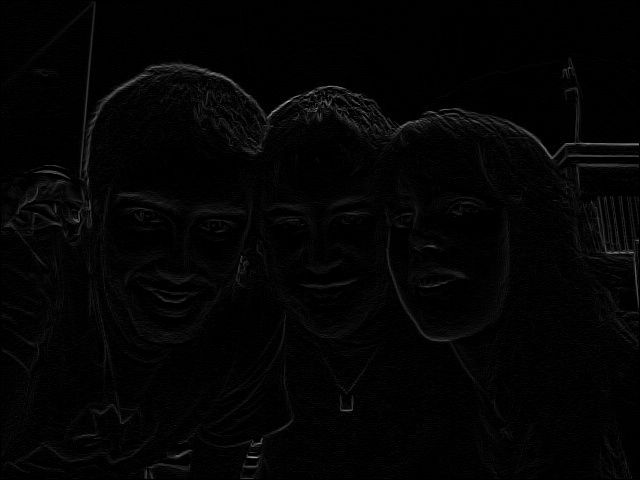
\includegraphics[scale=0.30]{Graficos/out/roberts_foto3.jpg}
\end{center}


\subsection{Operador de Prewitt}

\begin{center}
	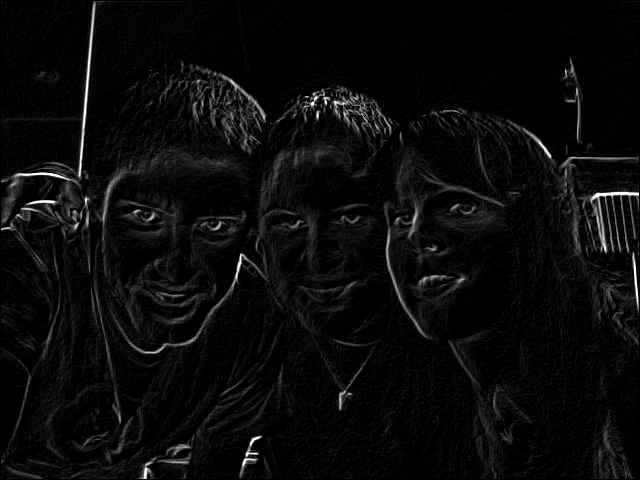
\includegraphics[scale=0.30]{Graficos/out/prewitt_foto3.jpg}
\end{center}

\subsection{Operador de Sobel}

\subsubsection{Derivaci\'on s\'olo en x}
\begin{center}
	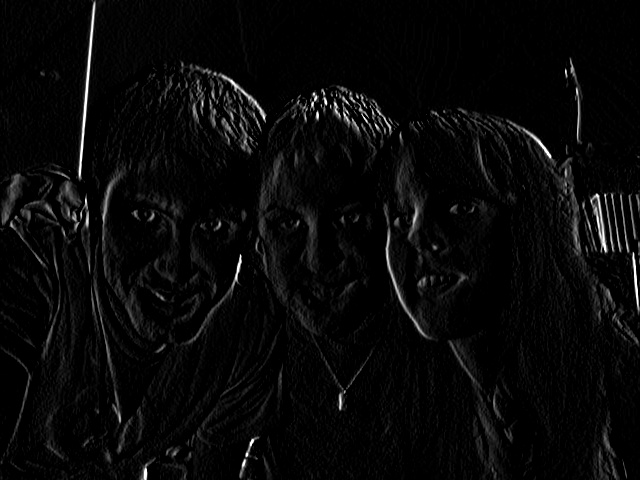
\includegraphics[scale=0.30]{Graficos/out/cvSobelX_foto3.jpg}
	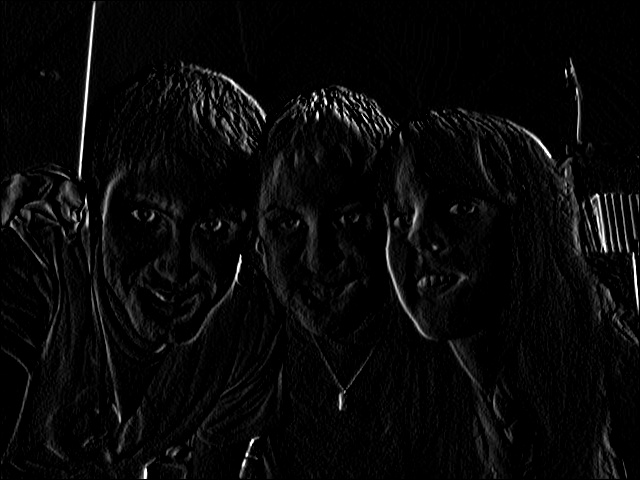
\includegraphics[scale=0.30]{Graficos/out/sobelX_foto3.jpg}
\end{center}

\subsubsection{Derivaci\'on s\'olo en y}
\begin{center}
	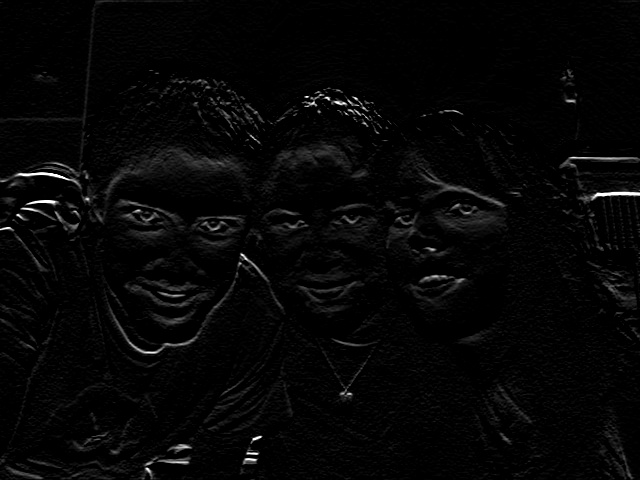
\includegraphics[scale=0.30]{Graficos/out/cvSobelY_foto3.jpg}
	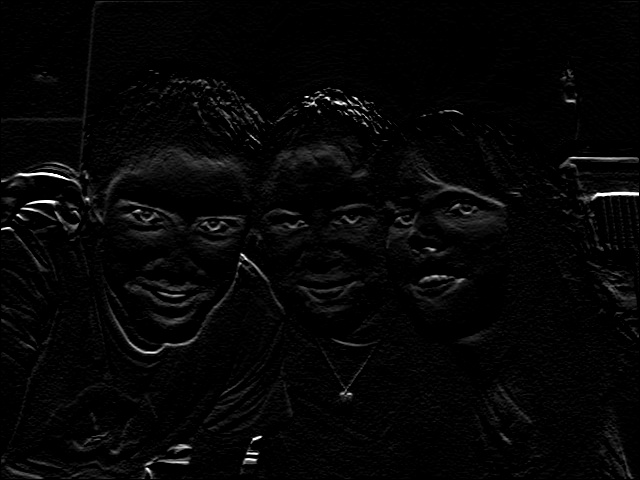
\includegraphics[scale=0.30]{Graficos/out/sobelY_foto3.jpg}
\end{center}

\subsubsection{Derivaci\'on en x y en y}
\begin{center}
	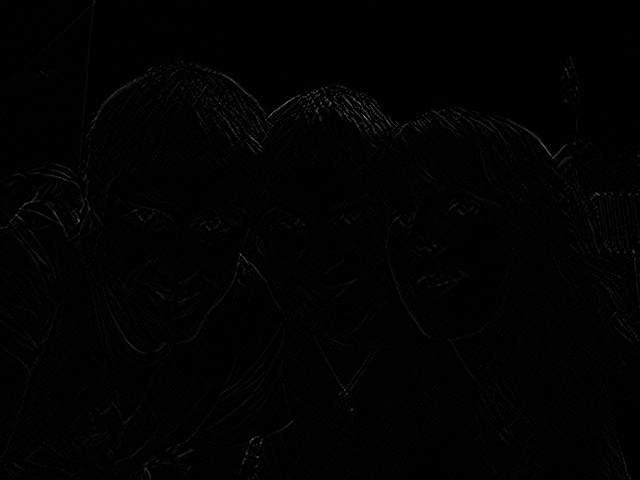
\includegraphics[scale=0.30]{Graficos/out/cvSobelXY_foto3.jpg}
	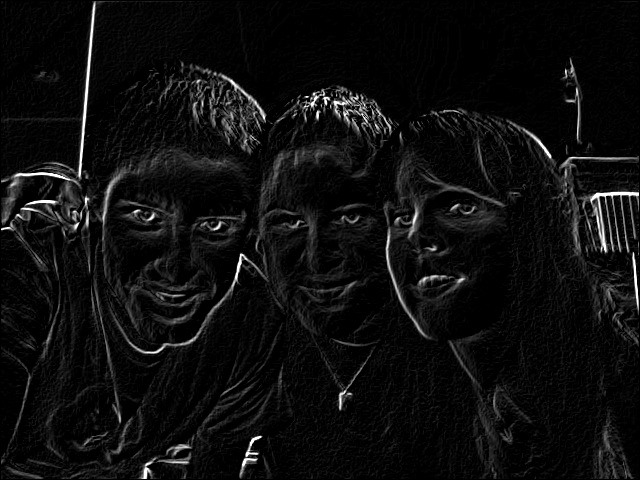
\includegraphics[scale=0.30]{Graficos/out/sobelXY_foto3.jpg}
\end{center}

En esta \'ultima comparaci\'on existe una gran diferencia entre la implementaci\'on de OpenCV (izquierda) y la nuestra (derecha).
Esto se debe a que la implementaci\'on de la librer\'ia no calcula la norma para la detecci\'on de bordes en XY, y eso hace que la saturaci\'on final de la im\'agen sea bastante m\'as oscura que la nuestra, y muy alejada a los bordes que la misma libreria detecto analizando particularmente.

\newpage

\section{Conclusiones}
Como conclusi\'on de este trabajo podemos destacar la importancia de optimizar un c\'odigo y las grandes diferencias que se aprecian al hacerlo. En este caso al procesar sobre una matriz y sabiendo los valores y el tama\~no de la misma pudimos ahorrar muchas operaciones gracias a no tener que realizar ningun ciclo. 
Por otro lado, cuando podiamos predecir una multiplicacion por 0, 1 o -1, aplicamos ciertas instrucciones que optimizaban el c\'odigo obteniendo el mismo resultado.
Se pierde portabilidad del algoritmo, pero se gana en velocidad.

\newpage

\section{Manual de usuario}
\begin{enumerate}
	\item Ejecutar el comando \texttt{make} o \texttt{make install} desde el directorio \texttt{tp1}.
	\item Acceder al directorio \texttt{exe} y ejecutarlo
	\begin{enumerate}
		\item Directo \texttt{./tp r1 images/lena.bmp }
		\item Interactivo \texttt{./tp }
	\end{enumerate}	
	\item Las im\'agenes procesadas se encuentran en el directorio \texttt{resultados}.
	\item En el directorio \texttt{src/images/} se encuentran algunas im\'agenes de ejemplo para procesar.
	\item Para agregar im\'agenes a procesar, estas deben ser agregadas al directorio \texttt{src/images/}.

\end{enumerate}

\section*{Archivos}
\begin{lstlisting}[language=SHELXL]
tp1/
|-- Makefile
|-- enunciado
|   `-- Enunciado.pdf
|-- exe
|-- informe
|   `-- Informe.pdf
|-- resultados
`-- src
    |-- Makefile
    |-- asmPrewitt.asm
    |-- asmRoberts.asm
    |-- asmSobelXY.asm
    |-- auxiliares.asm
    |-- images
    |   |-- 10mb.jpg
    |   |-- 1mb.jpg
    |   |-- 2mb.jpg
    |   |-- 5mb.jpg
    |   |-- emma.jpeg
    |   |-- foto3.jpg
    |   |-- foto_tp.jpg
    |   `-- lena.bmp
    `-- main.c	
\end{lstlisting}


\end{document}
